\documentclass[a4paper,12pt,final]{article}
% Pour une impression recto verso, utilisez plutôt ce documentclass :
%\documentclass[a4paper,11pt,twoside,final]{article}


\usepackage[utf8]{inputenc}
\usepackage[T1]{fontenc}
\usepackage[english,francais]{babel}
\usepackage[pdftex]{graphicx}
\usepackage{setspace}
\usepackage{hyperref}
\usepackage[french]{varioref}
\usepackage{easylist}
\usepackage{eurosym}
\usepackage{graphicx}
\usepackage{caption}
\usepackage{subcaption}
\usepackage{wrapfig}
\usepackage{floatrow}
\usepackage{fancyhdr}
\usepackage{nameref}
\usepackage{listings}
\usepackage{color}
\usepackage{chngpage}
\usepackage{amsmath}
\usepackage{multirow}

\newcommand{\reporttitle}{Développements logiciels autour de GDL}     % Titre
\newcommand{\reportauthor}{Nodar \textsc{Kasradze}} % Auteur
\newcommand{\reportsubject}{Stage de fin d'étude} % Sujet
\newcommand{\HRule}{\rule{\linewidth}{0.5mm}}
\setlength{\parskip}{1ex} % Espace entre les paragraphes

\hypersetup{
    pdftitle={\reporttitle},%
    pdfauthor={\reportauthor},%
    pdfsubject={\reportsubject},%
    pdfkeywords={rapport} {vos} {mots} {clés},%
    linktoc=all
}

\fancypagestyle{firststyle}
{
   \fancyhf{}
   \renewcommand{\headrulewidth}{0pt}
   \fancyfoot[C]{\thepage}
}


\fancypagestyle{newfancy}
{
\fancyhf{}
\fancyhead[R]{\itshape   \leftmark}
\fancyfoot[C]{\thepage}
\renewcommand{\headrulewidth}{0.5pt}
}

\setlength{\headheight}{14.5pt}

\definecolor{dkgreen}{rgb}{0,0.6,0}
\definecolor{gray}{rgb}{0.5,0.5,0.5}
\definecolor{mauve}{rgb}{0.58,0,0.82}

\begin{document}
  % Inspiré de http://en.wikibooks.org/wiki/LaTeX/Title_Creation

\begin{titlepage}

\begin{center}

\begin{minipage}[t]{0.48\textwidth}
  \begin{flushleft}
    
\includegraphics [width=30mm]{images/logo-cnrs.png} \\[0.5cm]
    %\begin{spacing}{1.5}
      \textsc{\large Centre national de la recherche scientifique}
    %\end{spacing}
  \end{flushleft}
\end{minipage}
\begin{minipage}[t]{0.48\textwidth}
  \begin{flushright}
    
\includegraphics [width=50mm]{images/siteon0.png} \\[0.5cm]
    \textsc{\large Observatoire de Paris}
  \end{flushright}
\end{minipage} \\[1.5cm]

\textsc{\Large \reportsubject}\\[0.5cm]
\HRule \\[0.4cm]
{\huge \bfseries \reporttitle}\\[0.4cm]
\HRule \\[1.5cm]

\begin{minipage}[t]{0.3\textwidth}
  \begin{flushleft} \large
    \emph{Auteur :}\\
    \reportauthor
  \end{flushleft}
\end{minipage}
\begin{minipage}[t]{0.6\textwidth}
  \begin{flushright} \large
    \emph{Responsable :} \\
    M.~Alain \textsc{Coulais}
  \end{flushright}
\end{minipage}

\vfill

\begin{minipage}[t]{0.48\textwidth}
  \begin{center}
    
\includegraphics [width=40mm]{images/logo-paris8.jpg} \\[0.5cm]
    \textsc{\large Université Paris 8}
  \end{center}
\end{minipage} \\[1.5cm]

{\large Année scolaire 2012-2013}

\end{center}

\end{titlepage}

   \pagestyle{empty}
  \cleardoublepage % Dans le cas du recto verso, ajoute une page blanche si besoin
  \begingroup
  \hypersetup{linkcolor=black}
  \tableofcontents % Table des matières
  \endgroup
  \sloppy          % Justification moins stricte : des mots ne dépasseront pas des paragraphes
  \cleardoublepage
  \pagestyle{firststyle}
  \section*{Remerciements}
\addcontentsline{toc}{section}{Remerciements}

Je tiens tout d’abord à remercier mon tuteur, monsieur Alain Coulais, sans qui ce stage n’aurait jamais eu lieu, pour sa gentillesse, ses conseils toujours plus qu’utiles, pour sa présence durant toute la durée de ce stage et enfin, pour tout l’enseignement qu’il a su m’apporter.



Je tiens à remercier monsieur Michel Caillat pour sa présence, sa gentillesse et pour toutes
les discussions passionnantes partagées.

Enfin je remercie l’ensemble du personnel du LERMA pour son accueil, sa gentillesse et sa bonne humeur, qui ont rendu mon séjour pendant le stage dans l'Observatoire de Paris des plus agréable.
  \cleardoublepage
  \section*{Résumé}
\addcontentsline{toc}{section}{Résumé} 

Mon stage s’est déroulé au sein du Laboratoire d'Etudes du Rayonnement et de la Matière en Astrophysique (LERMA) – Observatoire de Paris. Son but a été de contribuer au développement de GDL (clone libre d'IDL - logiciel largement utilisé en astronomie professionnelle) pour atteindre un niveau de maturité et de facilité d'utilisation garantissant la préservation à long terme des capacités de traitements et d'analyse pour de nombreuses expériences en astronomie au sol ou spatiale.

Ce stage était principalement destiné à la mise en place de:

1) fonctionnalités manquantes,

2) correction des bugs connus,

3) tests de régression et performance.


Ce stage nécessitait une connaissance solide du langage C++, car le projet GDL contient plus de 120 000 lignes écrites en ce langage. J'ai aussi eu à apprendre la syntaxe IDL/GDL pour pouvoir écrire des tests qui vont assurer la qualité des nouvelles fonctionnalités.


\section*{Summary}

I've done my internship at LERMA - Observatoire de Paris. The main goal was to contribute to GDL (free clone of IDL - very popular software in the domain of astronomy) to reach a level of maturity and usability ensuring long term preservation of analysis capabilities for numerous ground experiments and spaces missions based on IDL.

The course of internship was to implement:

1) missing functionalities,

2) correction of existing bugs,

3) performance and regression tests.

Solid knoledge of C++ language was necessary for this internship, beacause the GDL project contains more than 120 000 lines of code in that programming language. I've learned IDL/GDL syntaxe as well, that I've used to code the tests for ensuring the quality of recently implemented fonctionalities.

  \cleardoublepage
  \section*{Introduction} % Pas de numérotation
\addcontentsline{toc}{section}{Introduction} % Ajout dans la table des matières
  
La première année de master informatique à l’Université Paris 8 Vincennes-Saint-Denis se termine par un stage d’une durée minimum de 3 mois.
J'ai choisi de réaliser ce stage au sein du Laboratoire d’Études du Rayonnement et de la Matière en Astrophysique (LERMA) – Observatoire de Paris, situé à Paris 14ème. Les chercheurs de ce laboratoire travaillent avant tout à faire avancer le front des connaissances dans plusieurs axes de l'astronomie, notamment: la formation et l’évolution des galaxies, la formation de certaines étoiles, la chimie de la poussière interstellaire. Du logiciel libre est utilisé largement et est aussi produit: par exemple pour l'infrastructure de l'interféromètre ALMA et pour GDL destiné à être en libre accès pour tout le monde.
C’est ainsi que du 13 mai 2013 au 14 août 2013, je travaille sur un logiciel nommé GDL. Ce logiciel permet de faciliter le traitement des données. Ce projet utilise plusieurs bibliothèques open source, ce qui diminue le travail à réaliser et préserve l’utilisation de code testé pendant plusieurs années par une communauté ouverte.


Ma première approche sur ce projet a été de consacrer une première partie brève du stage à prendre en main les librairies utilisées tout en faisant les diverses installations qui me seront nécessaires pour la conception sur mon poste (GSL, Eigen, PLPlot, GraphicsMagick, …). Ensuite je prévoie une première ébauche de conception  me permettant mieux d’assimiler les bibliothèques, suivi d’une étude approfondie de besoin qui précède la conception spécifique de GDL.

Le travail effectué fut aussi réalisé à trois, avec mon tuteur de stage Alain Coulais et Mouadh Ayad, étudiant à l'Université Paris-Sud, IUT de Cachan et lui aussi stagiaire au LERMA travaillant sur un sujet complémentaire au mien, notamment l'élaboration d’une fonction SMOOTH et suite de tests de régression. En plus j'ai été en contact par courriel électronique avec Marc Schellens (fondateur et leader du projet GDL) et d'autres membres de la communauté. Le fait d’avoir travaillé en collaboration avec ces personnes a renforcé le cadre professionnel de ce stage car il est aujourd’hui impossible de travailler seul sur des projets de grande ou même petite envergure.


Dans la première partie de ce rapport je vais décrire le lieu du stage et l’environnement de travail. Après je vais présenter le cahier de charge et le but du stage. Dans la troisième et dernière partie je vais expliquer le travail que j’ai réalisé pendant ces trois mois, les difficultés que j’ai rencontrées, comment j’ai choisi de les résoudre et les résultats obtenus. Pour conclure le rapport, je résume les apports de ce stage, aussi bien personnels que professionnels.
  \cleardoublepage
  \pagestyle{newfancy}
  \section{Le cadre de travail}


\subsection{Observatoire de Paris}

L’Observatoire de Paris est un Grand Établissement sous tutelle du ministère de l’Enseignement supérieur et de la Recherche. Il a le statut d’EPSCP (Établissement public à caractère scientifique, culturel et professionnel). Ses trois missions principales sont : 1) la recherche, en contribuant au progrès de la connaissance de l’Univers par l’acquisition de données d’observation, le développement et l’exploitation des moyens appropriés, l’élaboration des outils théoriques nécessaires, 2) la formation initiale et continue, 3) la diffusion des connaissances. L’Observatoire de Paris abrite l’École Doctorale Astronomie et Astrophysique d’Île-de-France.

L’Observatoire de Paris compte un grand total d'environ 600 emplois permanents. Du coté MESR - 89 CNAP, 10 EC, 2 PRAG et 232 personnels de soutien; 248 titulaires du CNRS y sont affectés. L’Observatoire a le statut d'université et dispense un enseignement universitaire de haut niveau en astronomie et astrophysique allant du master au doctorat, avec possibilité de formation à distance, 245 étudiants y sont inscrits (ce chiffre intègre les étudiants des universités partenaires); par ailleurs 35 enseignants-chercheurs d’autres établissements de l’enseignement supérieur et 9 personnels divers travaillent dans les laboratoires de l’établissement; l’établissement emploie 42 contractuels dont 11 sur postes vacants, 19 sur contrat CNRS, le reste sur budget de l’établissement; son budget annuel hors salaires est de 20 M\euro\ et sa masse salariale est estimée à 35 M\euro.

\begin{figure}[!ht]
    \centerline{
    	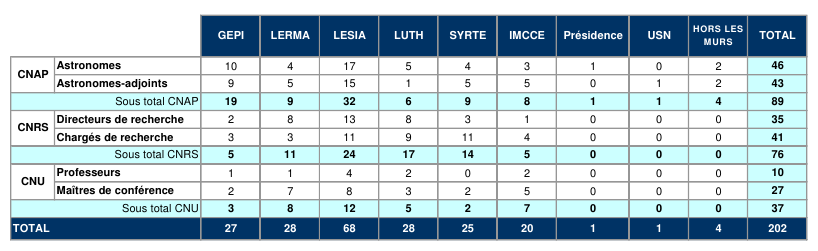
\includegraphics[width=1.3\textwidth]{./images/repartition_effectif.png}
    	}
    \caption{Répartition des effectifs (chercheurs et EC) par composante et par corps}
	%\centerline{}
		%\centerline{Source - Bilan Sociale 2010 http://ca.obspm.fr/IMG/pdf/09_Bilan-social-2010.pdf}
    \label{repartition_effectif}
\end{figure}

Cette institution représente le plus grand pôle national de recherche en astronomie. Il a été fondé en 1667. Près d’un tiers (30 \%) des astronomes français y poursuivent leurs recherches au sein de sept laboratoires situés sur trois campus (Paris fondé en 1667 par Louis XIV, Meudon fondé en 1876 par Jules Janssen dans des bâtiments du château de Meudon et Nançay construit en 1953 sur un terrain de l’ENS).

Il existe un partenariat fort entre l’Observatoire et le CNRS/INSU car les laboratoires de recherches sont tous des “Unités mixtes de recherche” et, souvent, en rattachement secondaire à d’autres universités scientifiques.

Les activités de recherche de l’Observatoire de Paris sont structurées autour de:


\begin{itemize}
\item[$\bullet$] 5 UMR associées au CNRS:
	\begin{itemize}
	\item GEPI: Galaxies, Étoiles, Physique et Instrumentation
	\item LERMA: Laboratoire d’Études du Rayonnement et de la Matière en Astrophysique
	\item LESIA: Laboratoire d’Études Spatiales et d’Instrumentation en Astrophysique
	\item LUTH: Laboratoire Univers et Théories
	\item SYRTE: SYstèmes de Référence Temps Espace
	\end{itemize}
\item[$\bullet$] 1 institut qui est aussi une UMR CNRS:
	\begin{itemize}
	\item IMCCE: Institut de mécanique céleste et de calcul des éphémérides
	\end{itemize}
\item[$\bullet$] 1 unité de service et de recherche:
	\begin{itemize}
	\item La station radioastronomique de Nançay
	\end{itemize}
\item[$\bullet$] 1 laboratoire de recherche associé ayant pour tutelle principale l’Université de Paris-Diderot, Paris 7:
	\begin{itemize}
	\item APC: AstroParticule et Cosmologie
	\end{itemize}
\item[$\bullet$] 1 unité mixte de service, créée en 2002, qui regroupe les services communs et centraux.
\item[$\bullet$] 1 unité de Formation et Enseignement\\
\end{itemize}

%\newline
\newpage
\subsection{Matériels utilisés}
J'ai utilisé divers ordinateurs, de l'ordinateur personnel (PC sous Linux) à des serveurs multi-cœurs avec des dizaines d'usagers, tout au laboratoire qu'à la DIO.

La DIO (Division Informatique de l’Observatoire) est un service chargé de tous les aspects informatiques mutualisés de l’Observatoire de Paris: système et réseau, calcul, stockage ainsi que du système d’information, de la bureautique des services centraux et de l’infrastructure technique de l’Observatoire virtuel.

Pour accéder aux services numérique gérés par la DIO un compte LDAP m'a été créé. Via ce compte je pouvais aussi accéder au courriel electronique (@obsmp.fr) et au réseau sans-fils interne. Ce compte LDAP permet aussi d'atteindre le réseau interne via un rebond SSH sur un des deux "firewall" (physiquement 1 à Meuden et 1 à Pais).\\

Le travail a été effectué sur une machine personnel, et des serveurs du LERMA et de la DIO:\\

\begin{itemize}
\item \textsc{\Large aramis}

	un serveur sous CentOS Linux version 5.9,\\
	avec 8 c\oe urs (deux Intel\textregistered\ Xeon\textregistered\ CPU           X5450  @ 3.00GHz)  64 bits\\
	et 16 Go de mémoire vive.
	\\
\item \textsc{\Large m2paris} (DIO UFE)

	un serveur sous Debian Linux version 7,\\
	avec 16 c\oe urs (deux Intel\textregistered\ Xeon\textregistered\ CPU           L5520  @ 2.27GHz)  64 bits\\
	et 12 Go de mémoire vive.
	\\
\item \textsc{\Large medusa}

	un serveur sous CentOS Linux version 5.9,\\
	avec 48 c\oe urs (quatre AMD Opteron\textregistered\  6176 SE @ 2.3GHz) 64 bits\\
	et 128 Go de mémoire vive.
	\\
\item \textsc{\Large haka}

	une machine personnelle sous Ubuntu Linux version 12.04.2,\\
	avec Intel\textregistered\ Core\textregistered 2 CPU          6400  @ 2.13GHz  32 bits\\
	et 2 Go de mémoire vive.
\end{itemize}



\begin{figure}
        \centering
        \begin{subfigure}[b]{0.5\textwidth}
                \centering
                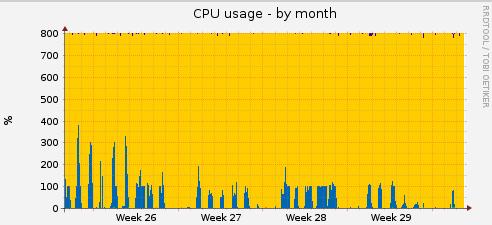
\includegraphics[width=\textwidth]{./images/aramis-cpu-monthm.png}
                \caption{\textsc{\large aramis}}
                %\centerline{Source - https://sionet.obspm.fr/munin/lerma-a111/aramis/cpu-month.png}
                \label{aramis}
        \end{subfigure}%
        ~
        \begin{subfigure}[b]{0.5\textwidth}
                \centering
                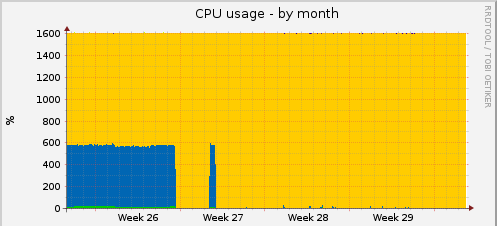
\includegraphics[width=\textwidth]{./images/m2paris-cpu-monthm.png}
                \caption{\textsc{\large m2paris}}
                %\centerline{Source - https://sionet.obspm.fr/munin/ufe/m2dsg-pro.obspm.fr/cpu-month.png}
                \label{m2paris}
        \end{subfigure}
        
        \begin{subfigure}[b]{0.5\textwidth}
                \centering
                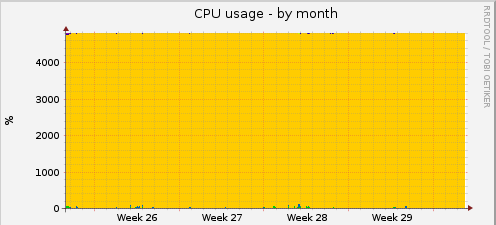
\includegraphics[width=\textwidth]{./images/medusa-cpu-monthm.png}
                \caption{\textsc{\large medusa}}
               %\centerline{Source -  https://sionet.obspm.fr/munin/lerma-b15/medusa/cpu-month.png}
                \label{medusa}
        \end{subfigure}
        \caption{La charge des serveurs pour le mois de juillet 2013 vu par l'outil Mumin}\label{charge_serveurs}
        \label{charge}
\end{figure}
\newpage
J'utilisais la machine personnelle (\textsc{\large haka}) pour connecter aux autres machines plus puissantes.
Compiler un projet, tel que GDL qui contient plus de 120 000 lignes de codes sur un machine comme \textsc{\large haka} va prendre environ 10 minutes, quand sur un serveur comme \textsc{\large aramis} la compilation va prendre au maximum 2 minutes quand la machine est partiellement chargée.

La charge des serveurs a été une des raisons d'avoir plusieurs machines à disposition, sur la Figure \ref{charge} on voit que la machine \textsc{\large aramis} est partiellement chargé (Figure \ref{aramis}), la machine \textsc{\large m2paris} est chargé de manière plus permanente (Figure \ref{m2paris}) et la charge de la machine \textsc{\large medusa} est négligeable (Figure \ref{medusa}). Le fait d'avoir à disposition des machines qui sont chargés a ses avantages, bien sur la majorité de travail est fait sur une machine avec la charge insignifiante pour diminuer le temps de compilation. Dès que la correction de code est terminé il faut tester le logiciel dans des environnements variés pour conforter son comportement. Notamment la dépendance aux versions de GCC et les problèmes liées aux architectures (32/64 bits). Dans un environnement chargé a été trouvé le problème avec les nombres des threads de OpenMP défini dans GDL (plus de détailles dans le section \ref{num_thread}, page \pageref{num_thread}). 

L'autre a été l'exigence de tester son compatibilité avec des systèmes d'exploitations et des architectures variées.

\subsection{Logiciels utilisés}
Les systèmes d'exploitation que j'ai utilisés pendant le stage étaient les différentes distributions de Linux et parfois Mac OS X. Pendent le stage je travaillais uniquement en mode commande. Les logiciels les plus utilisés sont cités ci-dessous:


\begin{description}
  \item[GNU Compiler Collection (GCC)] \hfill \\
	Crée en 1987 \textbf{GCC} est un ensemble de compilateurs portés sur les majorités de systèmes d'exploitation (Linux, Unix, Windows etc\ldots) et de microprocesseurs (x86, AMD64, ARM, SPARC etc\ldots). Il a été créé par le projet GNU comme un compilateur de langage C, mais après quelques années de développement il est devenu beaucoup plus fonctionnel que juste un compilateur.\\
	Aujourd'hui \textbf{GCC} est très extensible et adaptable aux besoins des utilisateurs, il contient aussi les compilateurs pour nombreux langages de programmation, tels que C, C++, Objective-C, Java, Ada, Fortran et d'autres langages, plus ou moins connus. \textbf{GCC} est le compilateur fourni avec nombreux systèmes d'exploitation comme Linux, BSD, Mac OS X ou BeOS. La plupart des logiciels libres sont compilée avec \textbf{GCC}, car en plus d’être performant, il est libre au sens de la licence GNU GPL.\\
	D’après tout ça on comprend pourquoi on a choisi \textbf{GCC} comme compilateur pour le projet GDL.
	\\ \\
  \item[GNU Debugger (GDB)] \hfill \\
  \textbf{GDB} a été créé en 1988  par Richard Stallman comme le débogueur standard du projet GNU. Comme pour  \textbf{GCC} il existe des ports de \textbf{GDB}  sur différent types de microprocesseurs et systèmes d'exploitation, il supporte différents langages de programmation et il est distribué sous les termes de la licence GNU GPL.\\
  \textbf{GDB} propose de nombreuses fonctionnalités pour tracer et contrôler l’exécution d'un programme informatique pas à pas. On peut surveiller ou modifier (si il y a besoin) une variable interne, on peut aussi faire un appel à fonction, indépendant du comportement prévu dans le programme. \textbf{GDB}  permet le débogage distant selon gdbserver, qui est lancé sur la même machine que le programme et le débogage est effectuer d'une autre. Cette technique est souvent utilisée pour déboguer un programme sur un système embarqué.
  \\ \\
  \item[Valgrind] \hfill \\
L'une des plus grandes difficultés de C++ est de gérer correctement la mémoire, alors pour diminuer les problèmes liés à la fuite de mémoire (l'absence de désallocation  de l'espace utilisé, double désallocation de l'espace utilisé etc\ldots) j'ai utilisé  \textbf{Valgrind}.\\
	A l'origine il a été crée comme un débogueur de mémoire pour Linux sur architecture x86, mais depuis il est devenue un plate-forme d'analyse dynamique pour les contrôleurs de la mémoire et "profilers". Il est disponible pour les systèmes d'exploitation Linux, Mac OS X et Android sur les microprocesseurs x86, x86-64, PowerPC et ARM. Grâce à sa licence GNU GPL v2,  il existe des ports non-officiels sur d'autres systèmes et architectures.\\
	Essentiellement \textbf{Valgrind} est un machine virtuelle utilisant la technique de compilation à la volée, le programme d'origine ne s’exécute pas directement sur un processeur, avant d’exécution il est traduit dans une représentation intermédiaire simplifié, les instructions sont ajoutées par un outil ("memcheck", "profiler" ou un outil externe) et finalement ces instructions sont traduites dans un code machine. A cause des procédures de traduction sous \textbf{Valgrind} l’exécution d'un programme est au moins 5 fois plus lent.\\
	Il est possible de combiner \textbf{Valgrind} avec \textbf{GDB} pour profiter des avantages de ces deux excellents outils.
\end{description}


\begin{figure}
        \centering
        \begin{subfigure}[b]{0.3\textwidth}
                \centering
    			
\includegraphics[width=0.4\textwidth]{./images/gcc.png}
                \caption{\textsc{GCC}}
				%\centerline{Source - http://upload.wikimedia.org/wikipedia/commons/thumb/a/a9/	Gccegg.svg/500px- Gccegg.svg.png}
                \label{logo-gcc}
        \end{subfigure}%
        ~
        \begin{subfigure}[b]{0.3\textwidth}
                \centering
                
\includegraphics[width=0.5\textwidth]{./images/gdb.png}
                \caption{\textsc{GDB}}
                %\centerline{Source - https://upload.wikimedia.org/wikipedia/commons/6/6a/Archer.jpg}
                \label{logo-gdb}
        \end{subfigure}%
        ~
        \begin{subfigure}[b]{0.3\textwidth}
                \centering
                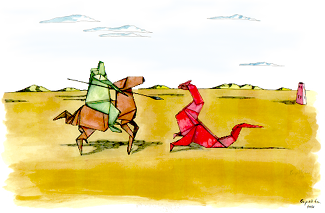
\includegraphics[width=0.7\textwidth]{./images/Valgrind_logo.png}
                \caption{\textsc{Valgrind}}
               %\centerline{Source -  https://upload.wikimedia.org/wikipedia/fr/f/f9/Valgrind_logo.png}
                \label{logo-valgrind}
        \end{subfigure}
        \caption{Les logos}\label{logos}
\end{figure}



  \cleardoublepage
  \section{Détails du sujet de stage}
\subsection{Présentation d'IDL}

\textbf{IDL} - Interactive Data Language est un langage interprété sous licence propriétaire. Créé en 1977 il a attiré l'attention des astronomes, médecins et d'autres scientifiques qui ont eu besoin d'un langage assez simple à apprendre et assez puissant pour traiter les données massives avec des fonctionnalités graphiques. La popularité d'\textbf{IDL} augmentait très vite à cause de ses fonctionnalités très pratiques pour les chercheurs, qui n'ont pas été programmeurs, mais qui ont besoin d'un outil pour faire des calculs scientifique. Entre ces fonctionnalités on trouve:

\begin{itemize}
	\item[$\bullet$] typage dynamique, le type est attribué automatiquement pendant la définition  de sa valeur (il y a une quinzaine de types);
	\item[$\bullet$] capacités d'un langage de programmation orientée objet;
	\item[$\bullet$] interprétation par machine virtuelle;
	\item[$\bullet$] affichage de tracés (1D, 2D, 3D) sans utilisation des bibliothèques graphiques externes;
	\item[$\bullet$] \textbf{IDL} est un langage vectorisé, les opérations sur scalaires sont généralisées pour pouvoir les utiliser sur les vecteurs, matrices et les tableaux à une dimension supérieure;
	\item[$\bullet$] multitâche, certaines fonctions et procédures sont parallélisés.
\end{itemize}

Grâce à ces avantages et une disponibilité sur les systèmes d'exploitations les plus utilisés y compris Windows, Mac OS X, Linux et Solaris, aujourd'hui il existe de nombreuses bibliothèques écrites complètement en syntaxe \textbf{IDL}. Ce sont les modules spécifiques à un domaine, qui ont été crées par les scientifiques pour simplifier l'utilisation de langage \textbf{IDL} dans ses domaines. Par exemple:  \textit{IDL Astronomy User's Library} ou plus court \textit{AstroLib} crée par Wayne Landsman. Cette bibliothèque contient des procédures fréquemment utilisées par les astronomes, notamment pour relire certaines formats de données (FITS).

\textbf{IDL} est un langage de programmation dont l’interpréteur du langage (ou compilateur) est propriétaire, ce qui signifie qu’il n’est pas libre. Cela signifie aussi que les scientifiques n’ont pas accès au code source et qu’il ne peuvent ouvrir qu’une quantité limitée de sessions au travers d’un système de jetons.

Le système de jetons dans \textbf{IDL} est contraignant. Déjà, l'abonnement pour un jeton par an coûte plus de 1000 \euro. En plus, il y a un nombre limité d’ouverture d’\textbf{IDL}, car à chaque démarrage du logiciel, ce dernier va réserver des jetons disponibles sur un serveur. Cela implique aussi que l’utilisateur doit rester connecté au serveur détenteur de jetons, ce qui peut très vite s’avérer compliqué en déplacement professionnel, durant des présentations ou lors de démonstration pendant des conférences.

Mais ce qui pose encore plus de problèmes aux scientifiques, c’est la pérennité du logiciel. En effet, ne pas avoir les codes source à disposition implique le fait que si la société en charge de garder le logiciel à jour décide de cesser ses activités, personne ne pourra continuer le développement. Dans le passé, la NASA et l'ESA ont contraint l’éditeur, qui voulait ne garder que Windows, à poursuivre le developpement sous Mac OS X et Linux. Or, la technique évolue tous les jours, et les logiciels tels qu'est \textbf{IDL} se doivent de la suivre. De plus, s’il n’est plus possible d’utiliser \textbf{IDL} dans le futur, les nombreuses bibliothèques écrites en syntaxe \textbf{IDL} deviendront inutiles et il faudra recoder tous les algorithmes dans un autre langage de programmation, ce qui serait très long et extrêmement cher. %\\

\subsection{Présentation de GDL}

\textbf{GDL} - GNU Data Language est un compilateur libre compatible avec la syntaxe \textbf{IDL}. Il a été créé par Marc Schellens en 2004 et il est développé par une communauté internationale de volontaires. \textbf{GDL} a été créé pour bénéficier des avantages d'\textbf{IDL} en ajoutant la liberté de compilateur pour assurer la pérennité de logiciel lui même et les bibliothèques tierces écrites en syntaxe \textbf{IDL}. L’interprétation de syntaxe est basé sur ANTLR.

\textbf{GDL} est déjà une alternative viable couvrant la plupart des fonctionnalités d'\textbf{IDL} et peut être utilisé pour compiler de larges "pipelines" de codes et bibliothèques en syntaxe \textbf{IDL}, lire les donnée de divers formats utilisées par les scientifiques (comme FITS, HDF, NetCDF, XDR), faire des calculs complexes et retourner un résultat exact. Grâce aux packagers les versions pré-compilées et pré-configurées sont mise à disposition pour les distribution de Linux les plus populaires (Debian, Ubuntu, Fedora, Gentoo, ArchLinux\ldots), FreeBSD et Mac OS X. Pour les utilisateurs plus expérimentés la version la plus récente du code est disponible sue un CVS (accès an lecture seul à tous), qui peut être compilée sur presque tous les systèmes basés sur Unix.

La compatibilité avec Windows n'est pas assurée, mais toutes les nouveau fonctionnalités prennent en compte la compatibilité avec ce système et les fonctionnalités déjà présent dans \textbf{GDL} continuent d'évoluer pour être compatibles avec tous les systèmes possibles.

\begin{figure}[!ht]
    \centerline{
    	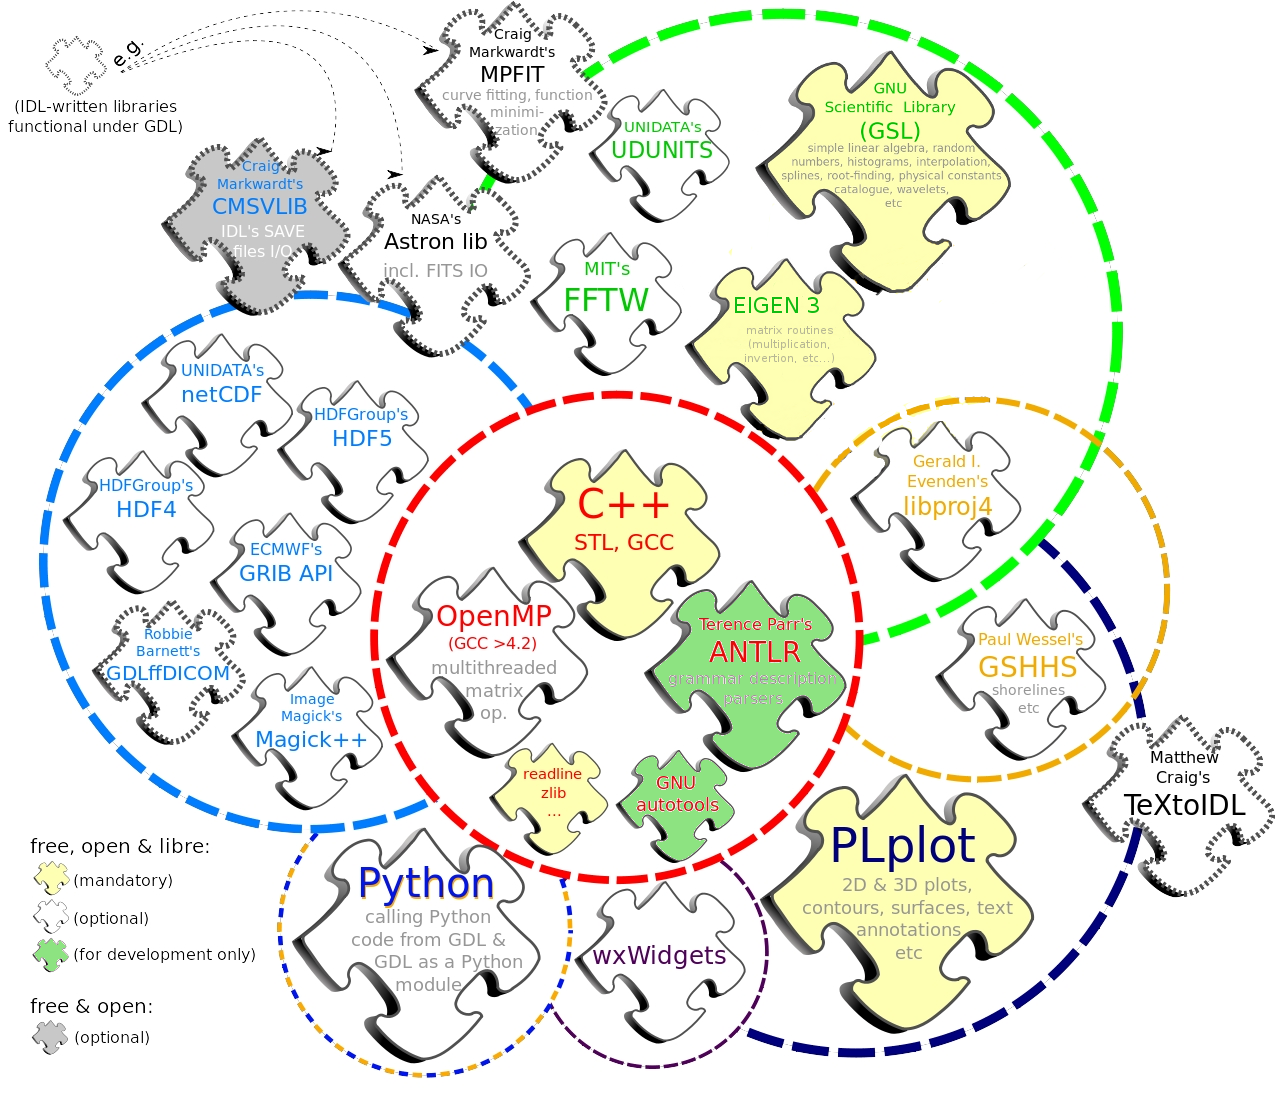
\includegraphics[width=1.3\textwidth]{./images/gdl-mod.png}
    	}
    \caption{Dépendances de GDL}
    \label{gdl-dep}
\end{figure}
%\newpage
Le choix de bonnes librairies externes et de bons algorithmes internes, l'usage de OpenMP, donnent une bonne performance globale à GDL. Sur les multi-cœurs, les gaines attendus sont généralement constatés. Les tests de performances actuels montrent que les calculs avec \textbf{GDL} sont aussi rapides (parfois plus vite), que les calculs avec son  adversaire propriétaire et ce, en respectant le gain par nombre de cœurs. L'ultime déficience connue dans le benchmarck de référence (IDL TIME\_TEST\_4) est SMOOTH, sujet du second stagiaire.
%\newpage
Le plus grand inconvénient de \textbf{GDL} est l'absence de plusieurs fonctions et procédures présentes dans \textbf{IDL}, alors ma mission a été de diminuer le nombre de ces fonctions/procédures manquantes et de tester ces nouvelles fonctionnalités en comparant les performances de \textbf{GDL} et d'\textbf{IDL}.

Le projet \textbf{GDL} utilise la licence GNU GPL v2/v3. Les bibliothèques tierces utilisée dans ce projet sont uniquement des bibliothèques libres (la notion d'un logiciel libre/licence libre est définie dans la section \ref{log_lib}, page \pageref{log_lib}) avec la licence GPL ou un autre, compatible avec GPL. Une exception unique concerne une fonctionnalité importante d'un format propriétaire de fichier interne à \textbf{IDL}. Il se trouve qu'une librairie externe open source à la licence incompatible avec la GNU GPL permet de gérer ce format. Il revient à l'utilisateur d'ajouter lui même ce code.



\subsection{Logiciel libre}
\label{log_lib}


La notion de Logiciel Libre (Free Software) est inventée par Richard Stallman dans le début des années 1980. Une première définition est publiée en 1986 par FSF (Free Software Foundation), une organisation américaine à but non lucratif, dont la mission mondiale est la promotion du logiciel libre et la défense des utilisateurs. Cette définition se traduit par une tente d'une licence définissant les droits et les devoirs des utilisateurs en s'appuyant sur le droit d'auteur (Copyright). Rarement, la FSF modifie la notion de Logiciel libre afin de la clarifier ou pour résoudre des questions portant sur des points difficiles. Les deux principales licences GNU GPL sont les versions 2 et 3.

Selon la dernière définition, un programme est un logiciel libre si, en tant qu'utilisateur de ce programme, vous avez les quatre libertés essentielles:

\begin{description}
	\item[liberté 0]  \hfill \\ %[$\bullet$] \textbf{liberté 0:} 
la liberté d'exécuter le programme, pour tous les usages;
	\item[liberté 1]  \hfill \\  %[$\bullet$] \textbf{liberté 1:} 
la liberté d'étudier le fonctionnement du programme, et de le modifier pour qu'il effectue vos tâches informatiques comme vous le souhaitez; l'accès au code source est une condition nécessaire ;
	\item[liberté 2]  \hfill \\ %[$\bullet$] \textbf{liberté 2:} 
la liberté de redistribuer des copies, donc d'aider votre voisin;
	\item[liberté 3]   \hfill \\ %[$\bullet$] \textbf{liberté 3:} 
la liberté de distribuer aux autres des copies de vos versions modifiées; en faisant cela, vous donnez à toute la communauté une possibilité de profiter de vos changements ; l'accès au code source est une condition nécessaire.
\end{description}



Pour protéger la [non]liberté d'un logiciel et les droit d'utilisateur il existe plusieurs type de licences. La FSF classe les licences en trois catégories :

\begin{itemize}
	\item[$\bullet$] les licences libres compatibles avec GPL;
	\item[$\bullet$] les licences libres non compatibles avec GPL;
	\item[$\bullet$] les licences non libres/propriétaires.
\end{itemize}

\begin{figure}[!ht]
    \centerline{
    	
\includegraphics[width=0.4\textwidth]{./images/GPLv3_Logo.png}
    	}
    \caption{Logo de GPL version 3}
    \label{logo-gpl}
\end{figure}
\begin{description}

\item[GNU General Public License]\hfill \\
La Licence Publique Générale GNU (GNU GPL ou GPL) est une licence des logiciels libres. Elle a été créé par Richard Stallman en 1989 pour permettre au grand nombre de projets de partager leur code source. C'est la licence le plus utilisée dans le monde de logiciels libres. La dernière version est "GNU GPL version 3" publiée en 2007. Ses termes autorisent l'utilisateur de logiciel sous licence GPL à: distribuer ce logiciel, le modifier, distribuer la version modifié. L'utilisateur n'est pas autorisé à: changer la licence, distribuer ce logiciel sans code source, commercialiser ce logiciel.

Ce ne signifie pas qu'on peut pas faire de l'argent avec les logiciels libres. L’entreprise multi-nationale Red Hat avec un chiffre d’affaire d'un milliard de dollars est dédiée aux logiciels libre et Open Source, qui a basé son modèle d'affaires sur la vente des services et supporte pour les logiciels libres, notamment le noyau Linux et le système d'exploitation RHEL (Red Hat Enterprise Linux).

\item[Berkeley software distribution license]\hfill \\
La licence BSD est une licence libre compatible avec la GPL. Ses termes sont moins restrictives que celles de GPL. Un logiciel sous licence BSD en différence de GPL peut être utilisé dans un autre projet commercial et l’accès au code source modifié n'est pas garanti.

\item[End User License Agreement]\hfill \\
Contrat de Licence Utilisateur Final est un licence non libre/propriétaire, ses termes sont définis par l’entreprise publiant le logiciel. Il est utilisé pour mettre les différent restrictions (restriction de distribution; restriction sur le nombre d'utilisateurs, qui peuvent utiliser ce logiciel).
\end{description}

  \cleardoublepage
  \section{Travail réalisé}
\label{p3}
\subsection{Les premiers pas}

Mon stage a commencé par mon immersion dans le projet GDL. Ma première tâche a
consisté à compiler le code source de GDL sur les différentes machines
(\textsc{\small HAKA, ARAMIS\ldots}) avec les différentes options (en
activant ou non certaines bibliothèques externes facultatives). Pour chaque
machine la procédure de compilation a été différente, car les versions de
logiciels/bibliothèques installés ont été différentes ou sur certaines machines
les logiciels/bibliothèques nécessaires pour la compilation n’étaient pas
installés du tout. Les deux cas veulent dire que ça va prendre encore plus du
temps de compiler un projet sur de telles machines. Trouver une version de
logiciel qui va être compatible avec des logiciels/bibliothèques déjà installé
ce n'est pas une tâche triviale d'autant que le projet GDL contient 5 bibliothèques
obligatoires et plus d'une dizaine de bibliothèques optionnelles.

Le build du projet GDL est effectué par \textit{Autotools}, mais dans la version
suivante 0.9.4 \textit{CMake} va remplacer \textit{Autotools}, ce changement est
déjà accompli dans la version CVS du projet. Pour mieux comprendre la raison
pourquoi le projet va abandonner \textit{Autotools} voici le bref description de
ces deux outils:

\begin{description}
\item[Autotools]\hfill \\
Autotools (ou GNU build system) est un ensemble des projets GNU utilisés pour le build de projet sur différents systèmes d'exploitations basés sur Unix; ces outils peuvent être utilisés sur Windows, mais c'est une procédure très restrictive (compilation est possible seulement avec GCC) et prend plus de temps. Il est basé sur shell script, alors il ne nécessite pas l’installation des outils \textit{Autotools} pour faire un build. Ces outils sont très populaires dans le monde Linux. Les outils \textit{Autotools} ont de nombreux inconvénients à cause desquels les développeurs cherchent d'autres solutions. Les problèmes qui repoussent des programmeurs sont:
\begin{itemize}
	\item[$\bullet$] la syntaxe très compliquée, qui rend difficile l’écriture d'un
	script de configuration;
	\item[$\bullet$] large nombre des outils composant avec les syntaxes différents;
	\item[$\bullet$] les messages d'erreurs difficiles à comprendre;
	\item[$\bullet$] création de larges scripts de configuration même pour un
	projet basique;
	\item[$\bullet$] difficilement extensible, difficulté à rajouter des
	fonctionnalités non standard.
\end{itemize}

\item[CMake]\hfill \\
Cross Platform Make ou simplement \textit{CMake} est un moteur de production
créé dans le début des années 2000 pour être compatible avec divers plate-formes
(à peu près tous les systèmes basée sur Unix, Windows: Borland, Visual C++, cygwin\ldots) et divers environnements de développement (KDevelop, XCode, Visual Studio\ldots). Il devient un outils de plus en plus utilisé à cause de ces nombreux avantages:
\begin{itemize}
	\item[$\bullet$] ne dépend que d'un compilateur C++ quelconque;
	\item[$\bullet$] syntaxe très simple à apprendre;
	\item[$\bullet$] il génère un seul Makefile pour touts les plate-formes
	supportées;
	\item[$\bullet$] les messages d'erreurs aident à comprendre le problème;
	\item[$\bullet$] supporte le plate-forme des tests, qui facilite la création des suites des tests;
	\item[$\bullet$] la performance améliorée par rapport aux \textit{Autotools}.
\end{itemize}
Au début de projet GDL l'utilisation de  \textit{CMake} a été impossible à cause de sa licence non compatible avec GPL (GDL utilise la licence GPL), mais la migration sur la licence BSD a aidé à surmonter l'obstacle de non compatibilité. Le point le plus faible de \textit{CMake} représente sa documentation.
\end{description}

Par exemple, si on veut compiler sur \textsc {ARAMIS} la version CVS du projet,
on peut utiliser la suite des commandes suivants (au début on suppose qu'on
est dans la répertoire \textit{{\raise.17ex\hbox{$\scriptstyle\sim$}}/sources/gnudatalanguage/gdl/}):

\lstset{frame=tb,
  language=bash,
  aboveskip=3mm,
  belowskip=3mm,
  showstringspaces=false,
  columns=flexible,
  basicstyle={\ttfamily},
  numbers=none,
  morekeywords={mkdir, cmake, make},
  %numbersep=5pt,
  %numberstyle=\tiny\color{gray},
  rulecolor=\color{black},
  keywordstyle=\color{blue},
  commentstyle=\color{dkgreen},
  stringstyle=\color{mauve},
  breaklines=true,
  breakatwhitespace=true
  tabsize=3,
}

\begin{lstlisting}
mkdir compil build
cd compil
cmake .. -DHDF=OFF -DPSLIB=OFF -DPLPLOTDIR=~/sources/plplot-5.9.6/build/ 
-DCMAKE_INSTALL_PREFIX=~/sources/gnudatalanguage/gdl/build/ 
make -j 8
make check
\end{lstlisting}


\subsection{Fonction d'inversion de matrice}

\subsubsection{Contexte}

Ma première mission d’écriture de code a été le développement de la fonction
d'inversion de matrice. En fait la fonction d’inversion de matrice
(INVERT) était déjà présente dans le projet GDL, mais elle a été écrite en
utilisant la librairie GSL (GSL représente des outils de calculs numériques en
mathématiques appliquées, elle fait partie du projet GNU et est distribuée selon
les termes de la licence GNU GPL). Depuis début 2013, l’équipe GDL mène des essaies très fructueux avec la librairie Eigen. INVERT est un code important, il fallait voir si un gain de temps notable existe avec Eigen par rapport à la GSL. Alors j'ai dû réécrire INVERT en utilisant la librairie Eigen (librairie de C++ contenant des templates qui implémentent l’algèbre linaire et des opérations sur les matrices, sous la licence libre MPL2, qui représente l'hybride de BSD et GPL).

\subsubsection{Réalisation}
La philosophie de GDL est directement inspirée du monde libre, ainsi, si un code
existe déjà et qu’il est possible de l’intégrer dans le projet grâce à sa
licence, il est inutile de perdre du temps à le réécrire. On peut aussi choisir
entre plusieurs librairies externes en fonction de critères: simplicité,
taille, performance, évolution. C'est pourquoi, plutôt que de coder l’algorithme
d'inversion de matrice j'ai préféré utiliser les routines existantes et largement testées.

Dans la fonction d'inversion, la matrice est donnée sous les types du langage
C/C++. Pour mieux traiter les données Eigen a ses propres types de données et
pour convertir les donnée existant de type non-Eigen à un type interne d'Eigen
on a le mapping. La classe Map de bibliothèque Eigen contient des routines de
mapping. Ces routines sont trés simples à utiliser et elles sont très performantes.

Exemple de mapping:

\lstset{frame=tb,
  language=C++,
  aboveskip=3mm,ils
  belowskip=3mm,
  showstringspaces=false,
  columns=flexible,
  basicstyle={\ttfamily},
  numbers=none,
  morekeywords={Map,MatrixXf},
  %numbersep=5pt,
  %numberstyle=\tiny\color{gray},
  rulecolor=\color{black},
  keywordstyle=\color{blue},
  commentstyle=\color{dkgreen},
  stringstyle=\color{mauve},
  breaklines=true,
  breakatwhitespace=true
  tabsize=3,
}

\begin{lstlisting}
float array[rows*cols];
Map<MatrixXf> m(array,rows,cols);
\end{lstlisting}


\subsubsection{Tests}

Avant de publier dans le CVS la nouvelle fonction d'inversion d'une matrice il faut la bien tester. Les tests sont nombreux et divers: 

\begin{itemize}
	\item[$\bullet$] tests de justesse,
	\item[$\bullet$] tests de types,
	\item[$\bullet$] tests de correspondance avec la syntaxe IDL,
	\item[$\bullet$] tests de performance.
\end{itemize}

Ces tests sont nécessaires pour assurer la qualité de projet et d’éviter les problèmes dans le futur. Les résultats des tests de performance seront discutées dans la section suivante.

\subsection{Nombre de threads}
\label{num_thread}

\subsubsection{Contexte}
Quand la fonction d'inversion de matrice utilisant la librairie Eigen (INVERT\_EIGEN) a été prête, ses benchmarcks sur une machine chargée ont montré un résultat complètement différent de celui de la machine non chargée. Par rapport à IDL la même fonction d'inversion de matrice sur une machine non chargée a été plus rapide pour tous les types, mais sur la machine chargée (même s'il y a eu un seul cœur occupé et 15 disponibles) pour certaines types la performance a baissé de 10 fois ou même plus. D’après l'analyse de la documentation de la librairie Eigen et la consultation (par courriel électronique) avec les autres membres de la communauté (Marc Schellens, Gilles Duvert\ldots) on a trouvé que le problème est causé par le nombre de threads défini statiquement et indépendant de la charge de machine pour OpenMP (Eigen utilise OpenMP pour bénéficier des multi-cœurs).

Cette occasion a produit un devoir inattendu: j'ai dû écrire une fonction qui va définir le nombre de threads dynamiquement avant chaque exécution du GDL et cette fonction va prendre en considération la charge de la machine sur laquelle elle est exécutée.

\subsubsection{Réalisation}
Sous les systèmes d'exploitations basées sur Unix on calcule le nombre de threads optimal (\textit{suggested\_num\_threads}) par la formule suivante:

\begin{equation}
	\large
	suggested\_num\_threads=nbofproc-avload
   	\label{form:num_threads_u}
\end{equation}

Le nombre de processeurs sur la machine (\textit{nbofproc}) est connu pour OpenMP et c'est un simple appel à sa fonction interne. Alors, il nous reste de trouver la charge moyenne de la machine (\textit{avload}). La charge moyenne de la machine est définie comme un nombre réel de type X.XX (par exemple: \textit{avload}=2.64 sur une machine avec 8 processeurs virtuels, où 2 signifie, que deux processeurs sont entièrement occupés et .64 signifie, que le troisième est chargé partiellement; les cinq processeurs sont libres), de dernière(s) 1, 5 ou 15 minutes. Dans notre cas on a décidé d'utiliser le moyen de 5 derniers minutes, car une minute c'est un intervalle très court pour faire une conclusion sur la charge de la machine et 15 minutes c'est trop long (on veut pas prendre en compte la charge de la machine par un logiciel qui a déjà terminé son fonctionnement). Puisque le nombre de processeurs est un nombre entier et la charge moyenne est un nombre réel, la valeur de la charge moyenne est arrondi au plus proche.

Sous le système d'exploitation Windows le nombre de threads optimal est calculé par la formule un peu différente:
\begin{equation}
	%\Large
	suggested\_num\_threads = nbofproc - avload * nbofproc/100
  	\label{form:num_threads_w}
\end{equation}

La différence vient du format de présentation de charge de la machine, qui est représenté sous Windows comme un pourcentage d'occupation de tous les processeurs virtuels (par exemple: \textit{avload}=50 sur une machine avec 8 processeurs virtuels signifie que 4 processeurs sont occupés et les 4 restants sont libres).

Le code source de la fonction \textit{set\_num\_threads} est disponible dans l'Annexe \ref{code_num_threads} sur page \pageref{code_num_threads}.


\subsubsection{Étude des performances}
%\vspace{2\baselineskip}\vspace{-\parskip}

L’aspect très important dans la concurrence entre GDL et IDL c'est la performance, afin qu'ils sont utilisés pour les calculs scientifiques. Signifiant, que les données à traiter sont assez larges (par exemple: les matrices avec des dimensions supérieures à 200). La performance de la majorité des fonctions de GDL est très proche ou même meilleure que la performance d'IDL, mais pour attirer plus d'utilisateurs il faut avoir un meilleur indice de performance que IDL pour tous les fonctions sur tous les systèmes d'exploitations.

Pour trouver les indices de performance des différents fonctions d'inversion de matrice une suite de tests a été écrite, ces tests se composent de calcul du temps d'inversion des matrices aux très larges dimensions (255, 256, 300, 500). Les tests ont été faits sur \textsc{ARAMIS}, qui pour le moment de tests a eu 2 cœurs occupés en permanence par des autres processus. Cette condition a été idéale pour tester la performance de cette nouvelle caractéristique qui a été introduite par la fonction de définition de nombre de threads.

D’après les tests, la fonction d'inversion de matrice utilisant la bibliothèque Eigen donne une meilleur performance que celle utilisant la bibliothèque GSL. Mais sur une machine chargée les deux fonctions deviennent incomparable avec la fonction de IDL, qui est largement plus rapide. Alors, après la fonction \textit{set\_num\_threads} la performance de la fonction d'inversion de matrice avec GSL (qui est utilisé dans la plupart de fonctions codés sous C++ pour les calcules scientifiques) est proche de la fonction présent dans IDL et parfois est meilleur.

Une fois les problèmes du nombre des threads optimale sont réglés, la fonction d'inversion de matrice avec Eigen a les meilleurs résultats pour touts les types (la Table \ref{test_perf} montre les temps de calcul pour les multiples fonctions). En plus d'une bonne performance, Eigen est simple à utiliser et il se charge de la gestion de la mémoire, qui dispense l'utilisateur de gérer les éventuelles fuites mémoire. C'est pourquoi Eigen a été choisi comme une bibliothèque pour les calculs matriciels pour les nouvelles fonctionnalités, qui vont faire partie de GDL version 0.9.4.\\

En conséquence, la définition dynamique du nombre de threads a permis d'obtenir un meilleur indice de performance pour l'inversion de matrice aussi bien que pour tous les fonctions utilisant la parallélisation avec OpenMP dès que les machines sont un peu chargées.

\renewcommand{\arraystretch}{1.3}
\begin{table}
\begin{center}
\renewcommand{\thefootnote}{\alph{footnote}}
    %\begin{adjustwidth}{-0.7in}{-1in}
    \begin{tabular}{  c | c | c | c | c | c |}
    \cline{2-6}
      & \multicolumn{2}{ | c | }{GDL INVERT\footnotemark[1]} & \multicolumn{1}{ | c | }{\multirow{2}{*}{IDL}} & \multicolumn{2}{ | c | }{GDL INVERT\footnotemark[2]} \\
    \cline{1-3}
    \cline{5-6}
    \multicolumn{1}{ |c| }{Type} 	& GSL 	& EIGEN &  		& GSL 	& EIGEN \\ \hline
    \multicolumn{1}{ |c| }{BYTE}	& 7.383 & 6.249 & 0.543 & 0.663 & 0.397	\\ \hline
    \multicolumn{1}{ |c| }{INT}		& 5.242 & 6.125	& 0.530 & 0.657 & 0.374	\\ \hline
    \multicolumn{1}{ |c| }{LONG} 	& 5.108	& 5.605	& 0.537 & 0.656 & 0.365	\\ \hline
    \multicolumn{1}{ |c| }{FLOAT} 	& 7.768	& 5.283	& 0.533 & 0.630 & 0.339	\\ \hline
    \multicolumn{1}{ |c| }{DOUBLE} 	& 5.645	& 6.580	& 1.161 & 0.690 & 0.466	\\ \hline
    \multicolumn{1}{ |c| }{COMPLEX} & 10.218& 9.467 & 3.991 & 2.004 & 1.651	\\ \hline
    \multicolumn{1}{ |c| }{DCOMPLEX} & 13.543& 2.675& 4.365 & 2.160 & 2.089	\\ \hline
    \multicolumn{1}{ |c| }{UINT} 	& 9.204	& 7.416 & 0.520 & 0.671 & 0.399	\\ \hline
    \multicolumn{1}{ |c| }{ULONG} 	& 5.546	& 5.238 & 0.522 & 0.666 & 0.397	\\ \hline
    \end{tabular}
        %\end{adjustwidth}
\end{center}
        
        \caption*{de
        \footnotetext[1]{sans \textit{set\_num\_threads} sur une machine chargé}
        \footnotetext[2]{avec \textit{set\_num\_threads} ou sans \textit{set\_num\_threads}, mais sur une machine non chargée}
        }
        \caption{Résultats des tests de performance sur la fonction INVERT, utilisant la GSL ou Eigen}
        \label{test_perf}
\end{table}



\newpage
\subsection{Factorisation de Cholesky}

\vspace{1\baselineskip}\vspace{-\parskip}

La tâche suivante a été de coder sous C++ la factorisation (décomposition) de
Cholesky d'une matrice. Dans IDL on a quatre procédures/fonctions concernant la
factorisation de Cholesky (CHOLDC, CHOLSOL, LA\_CHOLDC, LA\_CHOLSOL). Tous ces
procédures/fonctions étaient absentes dans GDL et des utilisateurs souhaitent en
bénéficier. Certaines codes en syntaxe IDL/GDL (PlanckSkyModel, iCosmo)
utilisent CHOLDC et ne pouvaient être totalement audités. Ma mission a été de
les rajouter en utilisant la bibliothèque Eigen.

Cette factorisation est utilisée pour la résolution des systèmes d'équations linéaires, simulations avec méthode de Monte-Carlo, filtre de Kalman, l'inversion d'une matrice hermitienne.\\

\subsubsection{Description de factorisation de Cholesky}

\vspace{1\baselineskip}\vspace{-\parskip}

La factorisation de Cholesky, nommée d'après André-Louis Cholesky, consiste, pour une matrice symétrique définie positive \textbf{A}, à déterminer une matrice triangulaire inférieure \textbf{L} telle que :
\begin{equation}
	%\Large
	A=LL^T
  	\label{form:cholesky}
\end{equation}

Ou \textbf{L\textsuperscript{T}} est la transposée de la matrice triangulaire inférieure \textbf{L}. On peut imposer que les éléments diagonaux de la matrice \textbf{L} soient tous positifs, et la factorisation correspondante est alors unique.\\

\begin{figure}[!ht]
    \centerline{
    	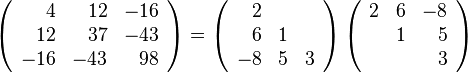
\includegraphics[width=0.8\textwidth]{./images/ex_chol.png}
    	}
    \caption{Exemple de factorisation de Cholesky}
	%\centerline{Source - http://upload.wikimedia.org/math/9/7/3/9733349e9de16e972daca756204d97db.png}
    \label{ex_chol}
\end{figure}

Pour la résolution d'un système d'équations linéaires, la factorisation de Cholesky est approximativement deux fois plus efficace que la décomposition LU. Alors c'est très important d'avoir dans GDL les routines concernant la factorisation de Cholesky.

\subsubsection{La réalisation de CHOLDC, CHOLSOL}

Le première ensemble de factorisation de Cholesky que j'ai codé a été la
procédure \textbf{CHOLDC}. Cette procédure est utilisée pour trouver une matrice
triangulaire inférieure d'une matrice symétrique définie positive donnée. Coder cette procédure a été une tâche sans peine, car j'ai déjà eu l’expérience de codage avec la librairie Eigen, que j'ai obtenu pendent ma mission précédent (la fonction d'inversion de matrice). En plus Eigen contient tous les algorithmes de suite de Cholesky, alors j'ai dû à faire la répartition des appels des algorithmes pour les types appropriés du coté de GDL.

Ensuite j'ai implémenté la fonction \textbf{CHOLSOL}. Cette fonction calcule la
solution pour un système d'équations linéaires \textbf{Ax=B}. Cette fonction
prend comme premier argument la matrice calculée par \textbf{CHOLDC}, mais GDL en différence d'IDL utilise la matrice triangulaire supérieure qui contient les valeurs initiales. La différence est à cause de librairie Eigen, qui ne support pas la résolution d'un système d'équations linéaires d’après les valeurs intermédiaires (la matrice décomposée). \\

\begin{figure}[!ht]
\centering
	\begin{subfigure}[b]{0.6\textwidth}
    	\centering
    		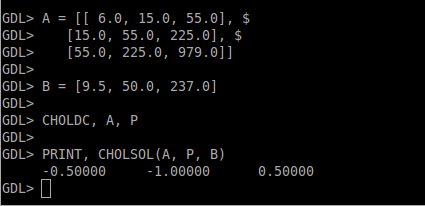
\includegraphics[width=\textwidth]{./images/ex_chols.png}
    		 \caption{GDL}
    		 \label{ex_chols_gdl}
    \end{subfigure}
    ~
    \begin{subfigure}[b]{0.6\textwidth}
    	\centering
    		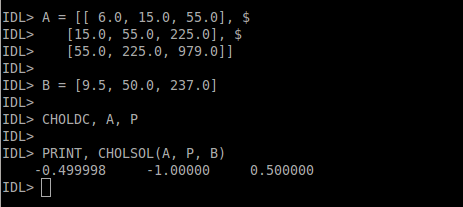
\includegraphics[width=\textwidth]{./images/ex_chols_idl.png}
    		\caption{IDL}
    		\label{ex_chols_idl}
    \end{subfigure}
    
    \caption{Exemple de résolution d'un système d'équations linéaires dans les interpréteurs GDL et IDL}
	%\centerline{Source - capture d'ecran}
    \label{ex_chols}
\end{figure}

La Figure \ref{ex_chols}\ montre un exemple de résolution d'un système
d'équations linéaires \textbf{Ax=B}\ dans différents interpréteurs en utilisant
la procédure \textbf{CHOLDC} et ensuite la fonction \textbf{CHOLSOL}. Pour
résoudre un système d'équations linéaires dans IDL on est obligé d’exécuter les
deux procédures, mais dans GDL on peut le résolve sans utilisation de
\textbf{CHOLDC}. Puisque dans la fonctions \textbf{CHOLSOL} on fait la
décomposition (c'est obligatoire en raison d'utilisation de la bibliothèque Eigen).
Pour assurer la compatibilité on peut résoudre \textbf{Ax=B}\ à la manière d'IDL
(suite de deux commandes).

La besoin de calculer deux fois la même factorisation baisse la performance de
GDL  dans résolution d'un système d'équations linéaires, mais GDL a un autre avantage par rapport à IDL: c'est une solution plus exacte. Dans un exemple qui est représenté sur la Figure \ref{ex_chols}\ la solution exacte est un vecteur avec les valeurs: \{ -0.500000, -1.00000, 0.500000 \} - ce que retourne GDL, mais le vecteur calculé par IDL est un peu différent, la première valeur contient un erreur de -0.000002.

\subsubsection{La réalisation de LA\_CHOLDC, LA\_CHOLSOL}

La procédure \textbf{LA\_CHOLDC} est la procédure \textbf{CHOLDC} généralisée
pour trouver la décomposition d'une matrice à coefficients complexes (matrice hermitienne). Pour la factorisation d'une matrice à coefficients réels, en plus de la formule \eqref{form:cholesky} (page \pageref{form:cholesky}) qui est utilisée par la procédure \textbf{CHOLDC}, \textbf{LA\_CHOLDC} peut utiliser la formule \eqref{form:cholesky-sup}, ou \textbf{U} est une matrice triangulaire supérieur et \textbf{U\textsuperscript{T}} est sa transposée:
\begin{equation}
	%\Large
	A=U^TU
  	\label{form:cholesky-sup}
\end{equation}

Pour une matrice hermitienne la procédure \textbf{LA\_CHOLDC} peut utiliser l'une des formules suivantes:

 \begin{equation}
	%\Large
	A=U^HU
  	\label{form:cholesky-com-sup}
\end{equation}

 \begin{equation}
	%\Large
	A=LL^H
  	\label{form:cholesky-com}
\end{equation}

\textbf{H} signifie une matrice adjointe (aussi appelée matrice transconjuguée).

La réalisation de \textbf{LA\_CHOLDC} a été similaire à la réalisation de
\textbf{CHOLDC}, car la bibliothèque Eigen gère les types complexes aussi bien que les autres types.

Le code complet des routines Cholesky est disponible dans le CVS du projet \url{http://smarturl.it/Cholesky}

\subsection{Convolution}
\subsubsection{Contexte}
La procédure \textbf{CONVOL} convole un tableau (1D, 2D, 3D\ldots) avec un noyau et retourne un tableau modifié. La convolution est largement utilisée dans divers domaines des sciences pour traitement d'image, traitement de signal, différenciation et beaucoup d'autres opérations. Le traitement d'images fait un grand partie d'astronomie, comme les image obtenu par les satellites parfois ont des défauts, on a besoin d'une procédure de correction. Alors c'est très important d'avoir la procédure de convolution dans GDL.


\begin{figure}[!ht]
    \centerline{
    	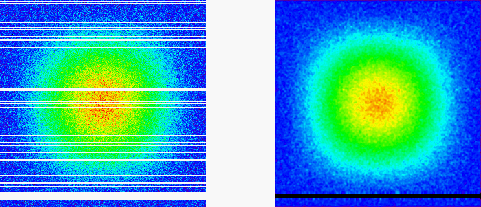
\includegraphics[width=0.8\textwidth]{./images/convol_example2.png}
    	}
    \caption{Exemple d'utilisation de convolution en traitement d'image en IDL. Cette fonctionnalité n'est pas encore disponible dans GDL}
	%\centerline{Source - http://www.exelisvis.com/docs/html/images/convol_example2.gif}
    \label{ex_convol_img}
\end{figure}

La Figure \ref{ex_convol_img} est un exemple de lissage d'image bruitée avec les données manquantes. Après la procédure de convolution la majorité des  données manquant est restauré et le bruit est réduit. On peut appliquer les différents effets sur cette image, l'effet est défini par le noyau (aussi appelé filtre) avec le-quelle image est convolé.

\begin{figure}[!ht]
\centering
	\begin{subfigure}[b]{0.3\textwidth}
    	\centering
    		
\includegraphics[width=\textwidth]{./images/ex_edge_or.png}
    		 \caption{Originale}
    		 \label{ex_edge_or}
    \end{subfigure}
    ~~
    \begin{subfigure}[b]{0.3\textwidth}
       	\centering
       		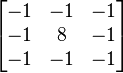
\includegraphics[width=\textwidth]{./images/filtre.png}
       		 \caption{Filtre}
       		 \label{ex_edge_fi}
    \end{subfigure}
    ~~
    \begin{subfigure}[b]{0.3\textwidth}
    	\centering
    		
\includegraphics[width=\textwidth]{./images/ex_edge_ch.png}
    		\caption{Après la convolution}
    		\label{ex_edge_ch}
    \end{subfigure}
        \caption{Exemple d'utilisation de convolution pour détecter les contours}
    \label{ex_edge}
\end{figure}

\subsubsection{Réalisation}
La fonction de convolution est présente dans GDL depuis 2004, mais elle est resté inchangée malgré les changements dans cette fonction dans IDL (nouveaux mot-clés ajoutés). D'ajouter la prise en compte effective de certaines nouveaux mot-clés dans \textbf{CONVOL} de GDL m'a été confié. J'ai commencé la mise à jour de cette fonction par regroupement de plusieurs fonctions concernant la convolution dans un même fichier. Cette stratégie est efficace pour le gain du temps et compréhension de vieux code afin qu'on ne cherche pas les parties du code.

Le code complet de fonction \textbf{CONVOL} avec tous les mot-clés déjà ajoutés est très large et la compréhension du code a pris beaucoup de temps. L’étude de code m'a pris environs une semaine. En plus des difficultés pour comprendre le code, comme il n'est pas en maintenance depuis longtemps la partie de code a perdu son efficacité. Donc, trouver les parties faibles du code et les corriger a fait la partie de cette mission.

Pendant la réalisation de mis à jour de la fonction de convolution la tâche le plus difficile a été d'assurer son fonctionnement pour tous les types. La grande partie du code est généralisé pour tous les types (en utilisant les Templates). Mais, comme les différents types ont différents caractéristiques on a eu besoin de réécrire la partie de la logique plusieurs fois en fonctionnement du type utilisé et pendant la compilation inclure le code approprié à ce type. Par exemple le fait que les nombres complexes n'ont pas d'ordre a causé des problèmes quand on a eu besoin de les comparer.

Le code de la fonction de convolution est dans l'Annexe \ref{code_convol}, page \pageref{code_convol}. Ce code ne représente pas le code complet de \textbf{CONVOL} de GDL, le code complet est disponible dans le CVS du projet \url{http://smarturl.it/Convol}

\subsubsection{Tests}

Des tests pour la convolution étaient absent dans la suite de tests du projet. Alors j'ai écrit des tests en syntaxe IDL/GDL pour assurer que tous les types sont bien gérés. Après l'application de ce test aux différents environnements, on a trouvé que les type \textbf{ULONG, ULONG64} ont des problèmes avec GCC version jusqu'à 4.4 et le projet ne compile pas. Pour l'instant ces deux types sont interdits dans \textbf{CONVOL}.

\subsection{Correction de bugs}

Pendant mon stage dans l’interval entre les grandes missions j'ai eu des "petit" tâches. Ces tâches comprennent la correction de divers bugs dans GDL. L'un de ces bug a été un problème typique du langage C++ - fuite mémoire (appel de \textbf{delete[]} pour libérer la mémoire alloué par \textbf{new}). Un autre crash de GDL était causé par la copie de bloc de mémoire de \textbf{long} à \textbf{double}. Ces deux types ont les longueurs différentes pour les différentes architectures (32/64 bits). Sur une architecture de 32 bits les deux ont la longueur maximale de 32 bits, mais sur l'architecture de 64 bits ils ont les longueurs différentes (\textbf{long} - 32 bits, \textbf{double} - 64 bits). Ces fuites mémoire ont été trouvées grâce au logiciel Valgrind.

J'ai aussi corrigé un bug dans le code de build en syntaxe CMake. Le projet GDL utilise les bibliothèques ImageMagick ou GraphicsMagic, la deuxième est plus prioritaire. CMake n'arrive pas à trouver si ImageMagick est installé dans un répertoire différent de celui par défaut. En analysant le code j'ai trouvé que le problème venait des versions récentes de ImageMagick ou le nom du répertoire a été changé. C'est un problème classique, quand les deux logiciels ne sont pas en accord.

Un dernier bug significatif concernait un traitement d'une chaîne de caractères dans GDL. Le traitement marchait jusqu'au premier espace blanc, j'ai ajouté une boucle pour passer toute la chaîne de caractères. Cette modification a amélioré les appels des commandes d'interpréteur de commandes système (par exemple: \textbf{cd, cp, mkdir \ldots}).










  \cleardoublepage
  \pagestyle{firststyle}
  \section*{Conclusion}
\addcontentsline{toc}{section}{Conclusion}

Le travail que j'ai réalisé lors du stage sur le projet GDL sera utilisé dans la prochain version du logiciel, qui va sortir à l'automne 2013. Ces corrections et améliorations vont aider GDL à devenir une alternative plus solide du logiciel propriétaire IDL (largement utilisé dans le domaine de l’astronomie). Tous les modifications sont mis dans le CVS et peuvent être téléchargées et compilées pour tester avant la sortie d'une version complète. Les utilisateurs ont déjà la possibilité de tester ces nouvelles fonctionnalités (les routines de Cholesky) et de ressentir la performance augmentée (grâce à la définition dynamique du nombre de threads pour OpenMP).\\

Ce stage au sein de l’Observatoire de Paris m'a été très profitable, et ce sur de nombreux plans. D'une part techniquement, j'ai pu découvrir un nouveau langage de programmation IDL/GDL, qui est un langage interprété. J'ai obtenu l’expérience de codage avec ce langage pendant que j'ai codé les différents tests de régression et de performance. Aussi j'ai approfondi mes connaissances en C++ durant plusieurs missions de correction de bugs et en ajoutant les nouvelles fonctionnalités dans GDL. Un autre apport de ce stage a été d'avoir utilisé plusieurs systèmes d'exploitation, qui m'a permis de me familiariser plus avec les différentes distributions de Linux (CentOS, Debian, Ubuntu). Ces systèmes étaient présents sur les serveurs aussi bien que sur les ordinateurs personnels.\\

Une des grandes difficultés techniques de ce stage fut d’avoir à modifier un code conçu et souvent modifié par d’autres personnes car il faut faire attention à bien comprendre pourquoi les développeurs précédents ont programmé de cette façon pour ensuite pouvoir apporter les modifications nécessaires. Mais le code qui n'est pas modifié pendent longtemps ne représente pas une logique triviale à comprendre non plus. En ce cas la difficulté est que l'auteur du code peut oublier la raison de choisir cette manière de codage. Dans tous les cas la difficulté du code augmente si le code n'est pas bien commenté et documenté. La documentation d'un logiciel est un aspect très important en informatique, car on a besoin d'utiliser les divers bibliothèques ou juste des petits morceaux du code de l'autre logiciel. Une bonne documentation facilite largement la vie des développeurs.\\  \\ \\

Les apports personnelles de ce stage sont tout aussi nombreux. Sur le plan professionnel, ce stage m’a apporté de nouvelles connaissances et a augmenté mes capacités de compréhension. Sur le plan humain, l’enrichissement est incontestable puisque j’ai pu développer mon indépendance et travailler en toute autonomie. J’ai par ailleurs pu juger de l’importance du relationnel entre les différents services, mais aussi entre les personnes internes à un service. Cette importance a dévoilé pendent les problèmes techniques (par exemple un problème avec la cable VGA), auxquelles la réaction a été très rapide et tout le monde a montré sa volonté d'aider.\\

Enfin, la communication fut un point important lors de ce stage. Le travail en équipe fait partie de la vie d’un ingénieur, ainsi, j’ai beaucoup appris de ce stage grâce au fait d’avoir travailler dans un laboratoire en collaboration avec un autre stagiaire. Aussi, le besoin de faire
des réunions pour faire le point sur l’avancement du projet s’est très vite fait ressentir afin de vérifier que les idées convergeaient et pour décider des suites à donner aux activités.


  \cleardoublepage
  \phantomsection\addcontentsline{toc}{section}{Références}

\begin{thebibliography}{ABC}	
    %\bibitem[REF]{reference} auteur. \emph{titre}. édition, année.
    %\bibitem[LPP]{lpp} Rolland. \emph{LaTeX par la pratique}. O'Reilly, 1999.
    
    \bibitem{william92}
       William H. Press, Brian P. Flannery.
      \emph{Numerical Recipes in C: The Art of Scientific Computing}.
      Cambridge University Press.
      2 edition.
      October 30, 1992.
    
    \bibitem{coulais10}
       Coulais, A.; Schellens, M.; Gales, J.; Arabas, S.; Boquien, M.; Chanial, P.; Messmer, P.; Fillmore, D.; Poplawski, O.; Maret, S.; Marchal, G.; Galmiche, N.; Mermet, T.
       \emph{Status of GDL - GNU Data Language}.
       434, Astronomical Data Analysis Software and Systems XIX.
       2010.
       \url{http://www.aspbooks.org/publications/434/187.pdf}
    
    \bibitem{coulais12}
       Coulais, A.; Schellens, M.; Arabas, S.; Lenoir, M.; Noreskal, L.; Erard, S.
       \emph{Space Missions: Long Term Preservation of IDL-based Software using GDL}.
       461, Astronomical Data Analysis Software and Systems XXI.
       2012.
       \url{http://www.aspbooks.org/publications/461/615.pdf}
    
    \bibitem{bilan10}
       \emph{Bilan Social}.
       L'Observatoire de Paris.
       Septembre 2010.
    
    \bibitem{rapport10}
       \emph{Rapport d’Évaluation de l’Observatoire de Paris}.
       Agence d’Évaluation de la Recherche et de l'Enseignement Supérieur.
       Mars 2010.
       \url{http://www.aeres-evaluation.fr/content/download/13342/186416/ffile/aeres-s1-obsparis.pdf}
    
    \bibitem{docgdl}
       Sylwester Arabas, Alain Coulais.
       \emph{Documentation de GDL}.
       Marc Schellens and The GDL team.
       Janvier 3, 2012.
       \url{http://gnudatalanguage.sourceforge.net/gdl.pdf}
    
    \bibitem{docidl}
       \emph{Documentation d'IDL}.
       \url{http://www.exelisvis.com/docs/}
    
    \bibitem{doceig}
       \emph{Documentation d'Eigen}.
       \url{http://eigen.tuxfamily.org/dox/}
    
    \bibitem{dio}
       \emph{Description de matériels de l'Observaoire de Paris}.
       \url{http://dio.obspm.fr}
    
    \bibitem{wiki}
       \emph{Les divers articles}.
       \url{http://wikipedia.org}
    
\end{thebibliography}

  \cleardoublepage
  \section*{Table des figures}
\addcontentsline{toc}{section}{Table des figures}


\begin{itemize}
	\item[$\star$]Source de Figure~\ref{repartition_effectif} sur la page~\pageref{repartition_effectif}:\\
	 				\nameref{repartition_effectif}\\ %Répartition des effectifs (chercheurs et EC) par composante et par corps\\
	 				\url{http://ca.obspm.fr/IMG/pdf/09_Bilan-social-2010.pdf}
	\item[$\star$]Source de Figure~\ref{aramis} sur la page~\pageref{aramis}:\\
					\nameref{aramis}\\ %La charge des serveurs pour le mois de juillet 2013 - \textsc{ARAMIS}\\
					\url{https://sionet.obspm.fr/munin/lerma-a111/aramis/cpu-month.png}
	\item[$\star$]Source de Figure~\ref{m2paris} sur la page~\pageref{m2paris}:\\
					\nameref{m2paris}\\ %\textsc{M2PARIS}\\
					\url{https://sionet.obspm.fr/munin/ufe/m2dsg-pro.obspm.fr/cpu-month.png}
	\item[$\star$]Source de Figure~\ref{medusa} sur la page~\pageref{medusa}:\\
					\nameref{medusa}\\ %\textsc{MEDUSA}\\
					\url{https://sionet.obspm.fr/munin/lerma-b15/medusa/cpu-month.png}
	\item[$\star$]Source de Figure~\ref{logo-gcc} sur la page~\pageref{logo-gcc}:\\
					\nameref{logo-gcc}\\ %\textsc{ GCC}\\
					\url{http://upload.wikimedia.org/wikipedia/commons/thumb/a/a9/	Gccegg.svg/500px- Gccegg.svg.png}
	\item[$\star$]Source de Figure~\ref{logo-gdb} sur la page~\pageref{logo-gdb}:\\
					\nameref{logo-gdb}\\ %\textsc{ GDB}\\
					\url{https://upload.wikimedia.org/wikipedia/commons/6/6a/Archer.jpg}
	\item[$\star$]Source de Figure~\ref{logo-valgrind} sur la page~\pageref{logo-valgrind}:\\
					\nameref{logo-valgrind}\\ %\textsc{Valgrind}\\
					\url{https://upload.wikimedia.org/wikipedia/fr/f/f9/Valgrind_logo.png}
	\item[$\star$]Source de Figure~\ref{gdl-dep} sur la page~\pageref{gdl-dep}:\\
					\nameref{gdl-dep}\\ %Dépendances de GDL\\
					Figure par Sylwester Arabas	
	\item[$\star$]Source de Figure~\ref{logo-gpl} sur la page~\pageref{logo-gpl}:\\
					\nameref{logo-gpl}\\ %Logo de GPL version 3\\
					\url{http://upload.wikimedia.org/wikipedia/commons/thumb/9/93/GPLv3_Logo.svg/500px-GPLv3_Logo.svg.png}
	\item[$\star$]Source de Figure~\ref{ex_chol} sur la page~\pageref{ex_chol}:\\
					\nameref{ex_chol}\\ %Exemple de factorisation de Cholesky\\
					\url{http://upload.wikimedia.org/math/9/7/3/9733349e9de16e972daca756204d97db.png}
	\item[$\star$]Source de Figure~\ref{ex_convol_img} sur la page~\pageref{ex_convol_img}:\\
					\nameref{ex_convol_img}\\ %Exemple d'utilisation de convolution dans traitement d'image\\
					\url{http://www.exelisvis.com/docs/html/images/convol_example2.gif}
	\item[$\star$]Source de Figure~\ref{ex_edge_or} sur la page~\pageref{ex_edge_or}:\\
					\nameref{ex_edge_or}\\ %Original\\
					\url{http://upload.wikimedia.org/wikipedia/commons/5/50/Vd-Orig.png}
	\item[$\star$]Source de Figure~\ref{ex_edge_fi} sur la page~\pageref{ex_edge_fi}:\\
					\nameref{ex_edge_fi}\\ %Filtre\\
					\url{http://upload.wikimedia.org/math/4/e/1/4e13c64b515f5d652e0b18c71d279425.png}
	\item[$\star$]Source de Figure~\ref{ex_edge_ch} sur la page~\pageref{ex_edge_ch}:\\
					\nameref{ex_edge_ch}\\ %Après la convolution\\
					\url{http://upload.wikimedia.org/wikipedia/commons/6/6d/Vd-Edge3.png}
\end{itemize}
  \cleardoublepage
  %\phantomsection\addcontentsline{toc}{section}{Abréviations}
\section*{Abréviations}
\addcontentsline{toc}{section}{Abréviations}

\begin{description} \itemsep3pt
  \item[ALMA]	Atacama Large Millimeter/sub-millimeter Array
  \item[ANTLR]	ANother Tool for Language Recognition
  \item[BSD]	Berkeley Software Distribution
  \item[CLI] 	Command Line Interface
  \item[CNAP]	Conseil National des Astronomes et Physiciens
  \item[CNRS]	Centre National de la Recherche Scientifique
  \item[CPU]	Central Processing Unit
  \item[CVS]	Concurrent Versions System
  \item[DIO]	Division Informatique de l’Observatoire
  \item[EC]		Enseignant-Chercheur
  \item[ESA]	European Space Agency
  \item[ENS]	École Normale Supérieure	
  \item[EPSCP]	Établissement Public à caractère Scientifique, Culturel et Professionnel
  \item[FITS]	Flexible Image Transport System
  \item[FSF]	Free Software Foundation
  \item[HDF]	Hierarchical Data Format
  \item[IDL] 	Interactive Data Language
  \item[INSU]	Institut National des Sciences de l’Univers
  \item[GDL] 	GNU Data Language
  \item[GPL]	General Public License
  \item[GSL] 	GNU Scientific Library
  \item[LDAP]	Lightweight Directory Access Protocol
  \item[MESR]	Ministère de l'Enseignement Supérieur et de la Recherche
  \item[MPL]	Mozilla Public License
  \item[NASA]	National Aeronautics and Space Administration
  \item[NetCDF]	Network Common Data Form
  \item[PRAG]	PRofesseur AGrégé
  \item[SSH]	Secure SHell
  \item[UMR]	Unité Mixte de Recherche
  \item[VGA]	Video Graphics Array
  \item[XDR]	External Data Representation
\end{description}
  \cleardoublepage
  \setcounter{subsection}{0}
\setcounter{page}{1}
\renewcommand{\thesubsection}{\Alph{subsection}} 
\renewcommand{\thepage}{\roman{page}}
\section*{Annexes}
\addcontentsline{toc}{section}{Annexes}
%\section{Annexes}


\lstset{frame=tb,
  language=C++,
  aboveskip=3mm,
  belowskip=3mm,
  showstringspaces=false,
  columns=flexible,
  basicstyle={\small\ttfamily},
  numbers=left,
  numbersep=5pt,
  numberstyle=\tiny\color{gray},
  rulecolor=\color{black},
  keywordstyle=\color{blue},
  commentstyle=\color{dkgreen},
  stringstyle=\color{mauve},
  breaklines=true,
  breakatwhitespace=true
  tabsize=3,
}


\subsection{Code de \textit{set\_num\_threads}}
\label{code_num_threads}

\lstinputlisting{./codes/set_num_threads.cpp}

\subsection{Fonction de convolution}
\label{code_convol}

\lstinputlisting{./codes/convol.cpp}
  
\end{document}

